\documentclass{article}

\usepackage{listings}
\usepackage{minted}
\usepackage{titlesec}
\usepackage{graphicx}
\usepackage{float}
\usepackage{mdframed}
\usepackage{xcolor}
\usepackage{xurl}

% Prevent word break at end of line
\tolerance=1
\emergencystretch=\maxdimen
\hyphenpenalty=10000
\hbadness=10000

\title{Evaluation task for Awkward Array GSoC project}
\author{Pratyush Das$^1$}
% https://tex.stackexchange.com/a/315873/193728
\date{%
    $^1$Institute of Engineering \& Management, Kolkata\\%
}

\begin{document}

\definecolor{light-gray}{gray}{0.95}

\maketitle

\begin{abstract}

    In this report, we demonstrate a sample GPU kernel designed to be an alternative to the CPU backend for array operations in the Awkward Array project. In particular, we implement a CUDA translation of the \textit{awkward\_listarray\_compact\_offsets} CPU kernel, and show how parallelizing the code on a GPU could significantly increase the speed of computation. The motivation of this report is to serve as an evaluation task to qualify to work on the project titled ``Awkward Array GPU kernels" under the mentorship of Jim Pivarski and David Lange.

\end{abstract}

\section{Introduction}

The sample CPU kernel (directly taken from the Awkward Array codebase) to be translated is defined below -
\begin{mdframed}[backgroundcolor=light-gray, roundcorner=10pt,leftmargin=0.5, rightmargin=0.5, innertopmargin=1,innerbottommargin=1, outerlinewidth=1, linecolor=light-gray]
\lstinputlisting[breaklines]{Code/cpukernel.c}
\end{mdframed}
Translating this particular CPU kernel serves as a good test because parallelizing this CPU kernel involves overcoming the loop carried dependency in the above code -
\begin{mdframed}[backgroundcolor=light-gray, roundcorner=10pt,leftmargin=0.5, rightmargin=0.5, innertopmargin=1,innerbottommargin=1, outerlinewidth=1, linecolor=light-gray]
\begin{lstlisting}
tooffsets[i + 1] = tooffsets[i] + (stop - start);
\end{lstlisting}
\end{mdframed}
where \mintinline{c}{tooffsets[i + 1]} depends on \mintinline{c}{toffsets[i]}.\\

The above algorithm can be visualized to illustrate its linear nature -
\begin{figure}[H]
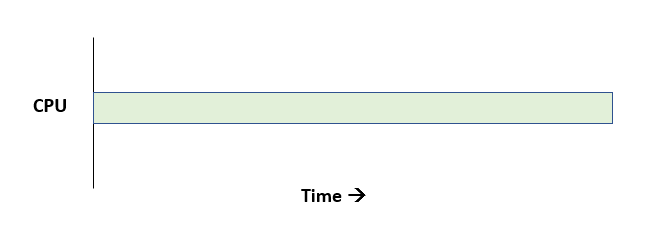
\includegraphics[width=\textwidth]{Graphics/cpu.PNG}
\caption{Visualizing sequential CPU algorithm}
\end{figure}


\section{Sequential algorithm on an Nvidia GPU}

\subsection{Sequential algorithm on a single thread}

\begin{figure}[H]
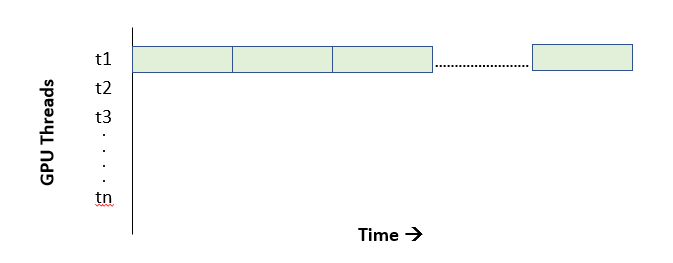
\includegraphics[width=\textwidth]{Graphics/naivesingle.PNG}
\caption{Visualizing GPU threads at work}
\end{figure}
\begin{mdframed}[backgroundcolor=light-gray, roundcorner=10pt,leftmargin=0.5, rightmargin=0.5, innertopmargin=1,innerbottommargin=1, outerlinewidth=1, linecolor=light-gray]
\lstinputlisting[breaklines]{Code/naivesinglefunc.cu}
\end{mdframed}
In the above code block\footnote{Full benchmarking code: \url{https://github.com/reikdas/GSoC-Proposal-2020/blob/master/testgsoc/naivesingle.cu}} we 

\subsection{Sequential algorithm on multiple threads}

\begin{figure}[H]
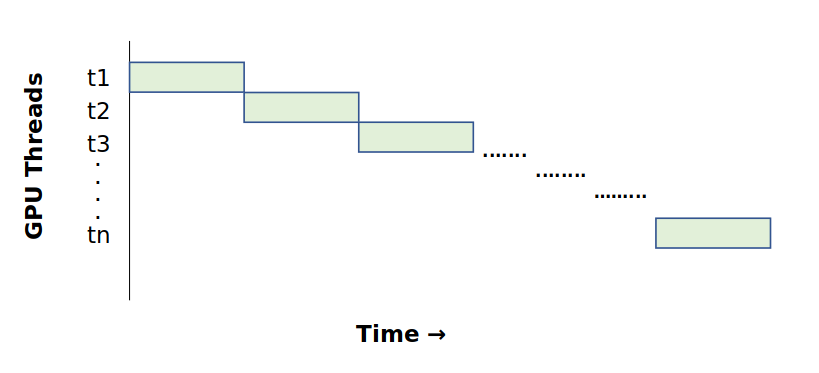
\includegraphics[width=\textwidth]{Graphics/naivemulti.PNG}
\caption{Visualizing GPU threads at work}
\end{figure}
\begin{mdframed}[backgroundcolor=light-gray, roundcorner=10pt,leftmargin=0.5, rightmargin=0.5, innertopmargin=1,innerbottommargin=1, outerlinewidth=1, linecolor=light-gray]
\lstinputlisting[breaklines]{Code/naivemultifunc.cu}
\end{mdframed}

\section{Parallel algorithm on an Nvidia GPU}

\begin{figure}[H]
\hfill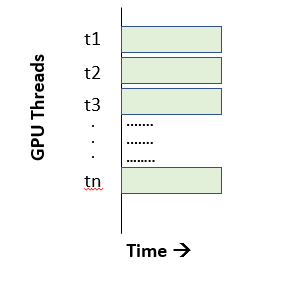
\includegraphics[scale=0.72]{Graphics/gpu.PNG}\hspace*{\fill}
\caption{Visualizing GPU threads at work}
\end{figure}
\begin{mdframed}[backgroundcolor=light-gray, roundcorner=10pt,leftmargin=0.5, rightmargin=0.5, innertopmargin=1,innerbottommargin=1, outerlinewidth=1, linecolor=light-gray]
\lstinputlisting[breaklines]{Code/thrustfunc.cu}
\end{mdframed}

\section{Benchmarks}

\section{Appendix}
We have only demonstrated the relevant CUDA kernels and not the surrounding code or main functions which are required to execute the kernels. The entire collection of complete code samples can be found in the GitHub repository.\par
In our full sample code which we have used for benchmarking, we have used 2 header files which includes helper functions to facilitate CUDA error checking in our code - \textit{helper\_cuda.h} and \textit{helper\_string.h}. Both of these helper header files are included in the NVIDIA CUDA SDK under the \textit{samples/inc/} folder. In the Awkward Array production code we might use the same CUDA error checking header files or we might decide to write our own CUDA error checking code.

\end{document}

